\documentclass{article}
\usepackage[utf8]{inputenc}
\usepackage{appendix}
\usepackage{url}
\usepackage{amssymb}    % for \checkmark
\usepackage{booktabs}  
\usepackage[most]{tcolorbox}


\title{Scenario Generation for Interactive Urban Environments}
\author{Paritosh Sharma, Hui-Yin Wu}
\date{September 2025}

\usepackage{graphicx}
\usepackage{hyperref}
\usepackage{pgfplots}
\usepackage{tikz}
\usepackage{amsmath}
\usepackage{multirow}
\usepackage{array}
\usepackage{enumitem}
\usepackage{lscape}
\usepackage{geometry} 
\usepackage{adjustbox}

\usetikzlibrary{shadows,arrows.meta,positioning,fit}

\tikzset{
  module/.style={rectangle, rounded corners=6pt, draw=orange!80!black, very thick, fill=black!90, 
                 text=white, align=left, font=\bfseries, minimum width=3.5cm, minimum height=2cm},
  subtext/.style={font=\scriptsize\color{white}, align=left},
  arrow/.style={-{Latex[length=3mm]}, thick, orange!80!black},
}

\tcbuselibrary{listings, breakable}

% Define a style for examples
\tcbset{
  examplebox/.style={
    colback=blue!3!white,
    colframe=blue!60!black,
    coltitle=black,
    fonttitle=\bfseries,
    sharp corners,
    boxrule=0.6pt,
    breakable,
    enhanced,
    left=5pt, right=5pt, top=5pt, bottom=5pt
  }
}

\begin{document}

\maketitle

\section*{Project members}

\begin{itemize}
    \item Scientific team: Paritosh Sharma, Hui-Yin Wu
\end{itemize}

\section{Context and objectives}

The document highlights the work plan for the the WP4 of the ANR Creative 3D~\footnote{\url{https://project.inria.fr/creattive3d/}} project. The expected outcome of this project is to create a generative model that is capable of creating personalized training scenarios in urban environments.

\section{Introduction}

Virtual Reality (VR) and Augmented Reality (AR) technologies have advanced significantly in recent years, enabling the creation of immersive and interactive environments for various applications. These can be further used to provide personalized training and rehabilitation scenarios. In the context of low vision rehabilitation, these models can be particularly useful to study pedestrian behaviours under normal and simulated vision. However, most simulated environments suffer from perceptual gaps between the designer, the user, and the system. The existing GUsT-3D framework~\cite{wu2022designing}, developed during the Creative3D project, provides a foundation to address this. However, the current framework is still limited by its reliance on a fixed set of urban environments and interactions innhibiting its ability to scale.

In parallel, recent works on 3D generative models for urban scenario generation has shown promising results in generating diverse and realistic urban environments. Additionally, these models have been able to capture the diverse nature and the complexities of an urban setting, including the interactions between pedestrians, vehicles, and the environment. Driven by these extraordinary capabilities, exploring the potential of generative models will enable us to create more diverse and realistic urban scenarios.

\section{Related Work}

In this section, we first start by reviewing prior work on pedestrian-in-the-loop simulations. Then, we review recent works on generative models for urban scenario generation as well as diffusion-based 4D generation. Finally, we discuss common validation methods used to evaluate the performance of these models.

\subsection{Pedestrian-in-the-Loop}

VR Simulations have been widely used to study pedestrian behavior and interactions in urban scenarios~\cite{wu2018using,tran2021review,mukoya2024jaywalkervr,schneider2020virtually}. This human-in-the-loop approach (also referred as pedestrian-in-the-loop\cite{hartmann2017pedestrian}) allows researchers to collect data on how pedestrians interact with their environment, including their decision-making processes, movement patterns, and responses to various stimuli. These simulations can be used to study a wide range of scenarios, from simple road crossings to complex urban environments with multiple interacting agents. More recently, JaywalkerVR~\cite{mukoya2024jaywalkervr}, a VR human-in-the-loop simulator, used CARLA~\cite{dosovitskiy2017carla} to create four different scenarios: jaywalking, parked cars, four-way stops, and parking lot entrances. Despite the obvious advantages, developing such simulators is still challenging because of the perceptual gaps between the designer, the user and the system as identified by Dourish~\cite{dourish2001action}.

The GUsT-3D framework~\cite{wu2022designing} addresses this by first defining the scene using a scenegraph, which captures the relationships between different elements in the scenario (ontology) and then defining the task to be carried out during the course of the scenario using a GUTasks (intersubjectivity). Lastly, it uses a query component for logging and post-scenario analysis of the experience (intentionality). This framework was also applied by creating a dataset of 6 road-crossing scenarios to study pedestrian behavior under normal and low vision~\cite{wu2023exploring}. Even though GusT-3D framework addresses the perceptual gaps which were identified by Dourish, it still relies on a fixed set of scenarios and interactions.

\subsection{Generative Models for Urban Scenario Generation}

\subsubsection{Image-based Generation}

Diffusion models have shown impressive results in generating high-quality images from textual descriptions. Models like DALL-E 2~\cite{ramesh2022hierarchical}, Imagen~\cite{saharia2022photorealistic}, and Stable Diffusion~\cite{rombach2022high} have demonstrated the ability to create diverse and realistic images based on text prompts. Recent works such as GameNGen~\cite{valevski2024diffusion}, Genie~\cite{bruce2024genie}, and DIAMOND~\cite{alonso2024diffusion} have shown the potential of diffusion models to generate game environments in real-time. However, these models suffer from latency issues since they are not truly 3D and generate image-by-image.


\subsubsection{Prompts}

Prompts are textual cues provided to the generative model to guide the scenario creation process. Since the popularity of LLMs like GPT-3, prompts have become a common way to interact with generative models. They can be used to specify the desired characteristics of the scenario, such as the type of environment, objects, and their relationships. Table \ref{tab:prompt_based_models} lists some of the recent prompt-based models for scenario generation.

\begin{table}[h]
\centering
\resizebox{\textwidth}{!}{
    \begin{tabular}{|c|c|c|}
    \hline
    \textbf{Model} & \textbf{Technique} & \textbf{Output} \\ \hline
    ScenicNL~\cite{elmaaroufi2024scenicnl} & Converts LLM Prompts to Scenic Constraints & Scenic Scenario \\ \hline
    ChatScene~\cite{zhang2024chatscene} & Conversational Agent for Scenario Definition using Scenic & Scenic Scenario \\ \hline
    LayoutGPT~\cite{feng2023layoutgpt} & Prompts converted to CSS-like Layout Formatting by LLMs & Layout Representation \\ \hline
    ChatDyn~\cite{wei2024chatdyn} & LLM-based planning and low-level trajectory generation for Pedestrian and Vehicle & 3D Scenario \\ \hline
    Work by Feng et al.~\cite{feng2025text} & JSON to describe layout and 3D models & 3D Scene \\ \hline
    TTSG~\cite{ruan2024traffic} & LLM-based planning and retrieval & 3D Scenario \\ \hline
    3D-SceneDreamer~\cite{zhang20243d} & Prompt to point-of-view image followed by image to 3D & 3D Scene \\ \hline
    GraphCanvas3D~\cite{liu2024graph} & Uses LLM to create a scenegraph and then a 3D scene & 3D Scene \\ \hline
    Scenethesis~\cite{ling2025scenethesis} & Uses LLM to create a scenegraph and then a 3D scene & 3D Scene \\ \hline
    SceneX~\cite{zhou2024scenex} & LLM to plan PCG (Procedural Controllable Generation) & 3D Scene \\ \hline
    Surreal Drivers~\cite{jin2024surrealdriver} & Chain-of-thought prompts & 3D Scene \\ \hline
    Text2nerf~\cite{zhang2024text2nerf} & Text prompts & 3D Scene \\ \hline
    X-Scene~\cite{yang2025x} & Text prompts & 3D Scene \\ \hline
    \end{tabular}
}
\caption{Prompt-based Models for Urban Scenario Generation}
\label{tab:prompt_based_models}
\end{table}

\subsubsection{Layout-guided Generation}

Layouts are structured representations of scenarios that capture the spatial relationships between different elements, such as buildings, roads, and pedestrians. These may include bird's-eye views, top-down maps, or other forms of spatial representations that provide a high-level overview of the scenario. Table~\ref{tab:layout_based_models} lists some of the recent layout-based models for scenario generation.

\begin{table}[ht]
\centering
    \begin{tabular}{|c|c|c|}
    \hline
    \textbf{Model} & \textbf{Technique} & \textbf{Output} \\ \hline
    CC3D~\cite{bahmani2023cc3d} & 2D Layout-based 3D Scene Generation & 3D Scene \\ \hline
    CityDreamer4D~\cite{xie2025citydreamer4d} & Uses a Layout Generator and a traffic scenario generator & 3D Scenario \\ \hline
    Infinicube~\cite{lu2024infinicube} & Text prompts, HD Maps and Bounding Boxes & 3D Scenario \\ \hline
    Work by Zhang et al.~\cite{urbandiff} & BEV map & 3D Scene \\ \hline
    UniScene~\cite{li2025uniscene} & BEV map & Multi-view video \\ \hline
    Savkin et al.~\cite{savkin2021unsupervised} & Scenegraph & Scenario Image \\ \hline
    \end{tabular}
\caption{Layout-based Models for Urban Scenario Generation}
\label{tab:layout_based_models}
\end{table}

Additionally, some works have also combined multimodal inputs with different types of data, prompts, layouts and other structured representations, to provide a richer context for scenario generation. Table~\ref{tab:multimodal_models} lists some of the recent multimodal models for scenario generation.

\begin{table}[ht]
\centering
\resizebox{\textwidth}{!}{
    \begin{tabular}{|c|c|c|}
    \hline
    \textbf{Model} & \textbf{Input Type} & \textbf{Output} \\ \hline
    CityX~\cite{zhang2024cityx} & Prompt, OSM file or Semantic Map & 3D Scenario \\ \hline
    CityCraft~\cite{deng2024citycraft} & Layout data and text prompts & 3D Scene \\ \hline
    Work by Liu et al.~\cite{liu2025controllable} & Scenegraph assisted using text prompts & 3D Scene \\ \hline
    GAUDI~\cite{bautista2022gaudi} & Conditioning using prompts or point-of-view images & 3D Scene \\ \hline
    MagicDrive3D~\cite{gao2024magicdrive3d} & Text prompts, Bird Eye View (BEV) map and 3D Bounding Boxes & Reconstructed 3D video \\ \hline
    Scene123~\cite{yang2024scene123} & Text prompt, point-of-view image or Text Description & 3D Scene \\ \hline
    StreetScapes~\cite{deng2024streetscapes} & BEV and height map with support for prompts & Video \\ \hline
    Urban Architect~\cite{lu2024urban} & 3D Layout and Text Prompts & 3D Scene \\ \hline
    Urban World~\cite{shang2024urbanworld} & Layout (generation) and prompts (refinement) & 3D Scenario \\ \hline
    Wonderplay~\cite{li2025wonderplay} & point-of-view image and action (physics) & 3D Video \\ \hline
    \end{tabular}}
\caption{Multimodal Models for Urban Scenario Generation}
\label{tab:multimodal_models}
\end{table}

\subsection{Validation}

Table \ref{tab:validation} lists common qualitative and quantitative validation methods used to evaluate the performance of generative models for urban road-crossing scenarios. These methods assess the quality, realism, and diversity of generated scenarios.

\begin{table}[ht]
\centering
\caption{Qualitative and Quantitative Evaluation Methods for Road-Crossing Scenarios}
\resizebox{\textwidth}{!}{
\begin{tabular}{|p{2.5cm}|p{3.5cm}|p{6.2cm}|p{4.5cm}|}
\hline
\textbf{Method Type} & \textbf{Evaluation Approach} & \textbf{Description} & \textbf{Use Case} \\
\hline

\multirow{5}{*}{Qualitative}
& Human Review & Human experts assess realism, scenario diversity, and layout plausibility. & Validates human-perceived quality and applicability of the scene. \\
\cline{2-4}
& Scenario Visualization & 3D visual inspection or rendered videos showing pedestrian, vehicle, and environment interactions. & Helps detect unrealistic or unnatural behavior/configurations. \\
\cline{2-4}
& Surveys & Collects subjective feedback on realism, perceived difficulty, or stress levels from participants. & Measures human-centric realism or emotional response. \\
\cline{2-4}
& Comparison & Compare scenario features (traffic density, gap opportunities, layout) to real-world statistics or distributions. & Validates realism by matching key scenario characteristics to empirical data. \\
\cline{2-4}
& Failure Cases & Identification and analysis of implausible or unsafe scenarios generated by the model. & Guides iterative model improvement. \\
\hline

\multirow{5}{*}{Quantitative}
& Scenario Feature Statistics & Statistical analysis of scenario properties (traffic speed, number/duration of gaps, crosswalk presence, etc.). & Ensures generated scenarios span realistic distributions. \\
\cline{2-4}
& Coverage and Diversity Metrics & Measures distributional entropy or spread of key attributes across all generated scenarios. & Assesses generalizability, scenario variety, and model's exploration of edge cases. \\
\cline{2-4}
& Criticality and Opportunity Metrics & Quantifies the frequency and severity of challenging situations (number of safe gaps, minimum feasible gap size, “no-go” cases). & Evaluates risk/challenge spectrum in the scenario catalog. \\
\cline{2-4}
& Sim2Real Gap (Domain Distance) & Computes metrics like KL-divergence, Earth Mover's Distance, t-SNE or FID/KID between generated and real scenario feature distributions. & Evaluates how closely synthetic scenarios match reality. \\
\cline{2-4}
& Controllability Metrics & Measures how well the model can generate scenarios based on prompts (CLIP, BLIP, VQA, etc.) & Assesses controllability and flexibility of the generative model. \\
\hline

\end{tabular}
}
\label{tab:validation}
\end{table}


%- Forecasting ? (AgentFormer)
%- XDE for agents?

\subsection{Code}

Currently tested code includes:

\subsubsection{Scenic}

Easy to setup and run on colab since the repository is well maintained.

\subsubsection{MagicDrive}

Had issues running due to model size and GPU memory limitations. Also realised only 2D video generation works for now since the code is not uploaded yet for 3D generation.

\subsubsection{MetaUrban/ScenarioNET}

Easy to setup and run since docker container is available and working.

\subsubsection{Threestudio}

Threestudio~\cite{liu2023threestudio} is a collection of 3D generative techniques. Easy to setup and run since docker container is provided. It is well maintained by the community and has a good documentation. Thus, good to test / refer different generative techniques for 3D.

\subsubsection{City Dreamer}

CityDreamer4D~\cite{xie2025citydreamer4d} tried testing the 3D branch with static scenes but encountered issues with the docker container.

\subsubsection{Urban Architect}

Urban Architect~\cite{lu2024urban} - Working. Can generate semantic maps and depth maps from a layout input. Which then can be used to generate the 3D scene. However, the code has to be adapted to generate using multiple GPUs due VRAM limitations.

\subsubsection{CLIP}

CLIP~\cite{radford2021learning} is a model that can be used to evaluate the quality of generated scenarios. Tested on colab with the pretrained ViT model.

\subsubsection{GraphDreamer}

GraphDreamer~\cite{gao2024graphdreamer} works but generation takes over 30 hours for 1 scenegraph. However, cannot generate complex scenes.

\section{Problem and Open Question}

%To add generative capabilities to frameworks like GUsT-3D~\cite{wu2022designing}, have demonstrated the use of scenegraphs and task specifications for pedestrian-in-the-loop simulations. However, these methods are limited in their ability to scale, as they lack generative capabilities needed to produce diverse and realistic scenarios. 
While recent generative models have demonstrated strong capabilities in synthesizing urban scenes from static layouts, they remain limited in their ability to model dynamic urban scenarios. In particular, they struggle to provide precise spatial and temporal control over objects and their interactions, which is essential for simulating a realistic traffic scenario.

This leads to the following open research question:

\textbf{How can we design a generative model that can create dynamic urban scenarios with precise spatial and temporal control over objects and their interactions?}

\section{Work Plan}

\subsection{Model Architecture}

Figure~\ref{fig:model_architecture} illustrates the proposed model architecture for generating dynamic urban scenarios. The model takes a scenario prompt as input, which is processed by a multimodal large language model (MLLM) to extract two key components: layout and tasks. Each component is then handled by specialized modules to generate the final 3D dynamic scene.

\begin{figure}[ht]
\centering
\resizebox{\textwidth}{!}{%
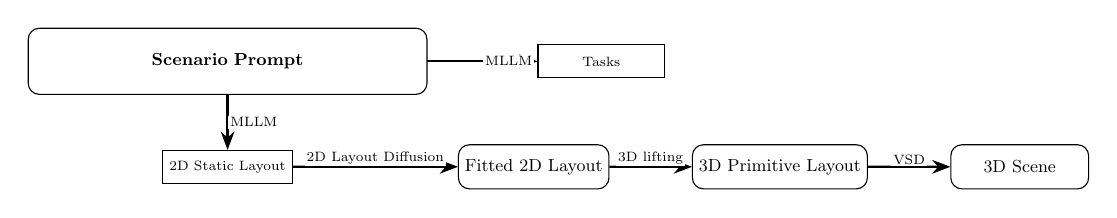
\begin{tikzpicture}[>=Stealth, node distance=0.6cm and 1cm, scale=0.7, transform shape]
  % Styles
  \tikzset{
    block/.style={rectangle, draw, rounded corners, align=center,
      minimum width=2.5cm, minimum height=0.8cm, font=\small},
    sub/.style={rectangle, draw, align=center,
      minimum width=2.3cm, minimum height=0.6cm, font=\scriptsize},
    arrow/.style={-Stealth, thick},
    panel/.style={draw,dashed, rounded corners, inner sep=0.2cm}
  }

  % ----- Panel (a): Input and Splitting -----
  \node[block, minimum height=1.2cm, text width=7cm, align=center] (input) {%
    \textbf{Scenario Prompt} \\[2pt]
  };

  % Three outputs below input
  \node[sub, below=1cm of input] (p2) {2D Static Layout};
  \node[sub, right=2cm of input] (p4) {Tasks};

  % ----- Panel (b): Static Scene Generator -----
  \node[block, right=3cm of p2] (c1) {Fitted 2D Layout};
  \node[block, right=1.5cm of c1] (c2) {3D Primitive Layout};
  \node[block, right=1.5cm of c2] (c3) {3D Scene};

  % ----- Arrows -----
  \draw[arrow] (input.south) -- node[right, font=\scriptsize, fill=white, inner sep=1pt] {MLLM} (p2.north);
  \draw[arrow] (input.east) -- node[right, font=\scriptsize, fill=white, inner sep=1pt] {MLLM} (p4.west);
  \draw[arrow] (p2.east) -- node[above, font=\scriptsize, fill=white, inner sep=1pt] {2D Layout Diffusion} (c1.west);
  \draw[arrow] (c1.east) -- node[above, font=\scriptsize, fill=white, inner sep=1pt] {3D lifting} (c2.west);
  \draw[arrow] (c2.east) -- node[above, font=\scriptsize, fill=white, inner sep=1pt] {VSD} (c3.west);

  % ----- Images below corresponding boxes -----
  %\node[left=0.4cm of p2] (img2) {\includegraphics[width=2.5cm]{images/gemini_static_example.png}};
  %\node[below=0.4cm of c3] (img1) {\includegraphics[width=2.5cm]{images/scene_example.png}};

\end{tikzpicture}%
}
\caption{Model Architecture}
\label{fig:model_architecture}
\end{figure}


\subsection{Input and Splitting}

Since no existing datasets provide paired text prompts with corresponding urban layouts and tasks, we propose leveraging the capabilities of MLLMs to parse and structure input prompts. Similar approaches have been explored in prior works, such as ChatDyn~\cite{wei2024chatdyn} for action planning, LayoutGPT~\cite{feng2023layoutgpt} for layout generation, and LLM-grounded Diffusion~\cite{lian2023llm} for LLM-conditioned image synthesis.

We first use a multimodal large language model (MLLM) (eg. Gemini) to process the input prompt and split it into the layout and tasks. The classes in the layout are based on the KITTI-360~\cite{liao2022kitti360} dataset. Here is an example of how the input prompt can be split:

\begin{tcolorbox}[examplebox, title=Scene Specification Format]

\textbf{Prompt}:

You are an urban scenario planning assistant. For the following urban scene prompt:\\

\emph{[Urban scene description goes here]}

\vspace{1em}
\noindent Generate a JSON object containing the following fields:
\begin{itemize}
    \item \textbf{static\_layout:} \\
    A $500 \times 500$ 2D layout map represented as an array of objects. Each object must include:
    \begin{itemize}
        \item \texttt{id}: unique identifier
        \item \texttt{type}: one of \{\texttt{pole}, \texttt{traffic sign}, \texttt{smallpole}, \texttt{lamp}, \texttt{trash bin}, \texttt{ground}, \texttt{road}, \texttt{sidewalk}, \texttt{parking}, \texttt{building}, \texttt{garage}, \texttt{fence}, \texttt{gate}, \texttt{vegetation}, \texttt{terrain}, \texttt{rail track}, \texttt{wall}, \texttt{box}, \texttt{vending machine}, \texttt{traffic light}, \texttt{rider}, \texttt{bicycle}, \texttt{motorcycle}, \texttt{motorbike}, \texttt{car}, \texttt{truck}, \texttt{bus}, \texttt{van}, \texttt{trailer}, \texttt{caravan}, \texttt{person}\}
        \item \texttt{position}: $(x, y)$ coordinates in meters within the 2D plane
        \item \texttt{orientation}: angle in degrees (0--360)
        \item \texttt{size}: width and height in meters
        \item \texttt{layer}: Layer classification for interactive scenarios. Choose from the default layers: 
        \begin{itemize}
            \item \textbf{Interactive layers:} 
            \begin{itemize}
                \item \texttt{"Container"}: Objects that can contain or hold other items (e.g., trash bins, boxes, bags)
                \item \texttt{"Support"}: Surfaces that can support objects being placed on them (e.g., tables, shelves, building roofs)
                \item \texttt{"Movable"}: Objects that can be moved or picked up (e.g., cars, people, bicycles, small objects)
                \item \texttt{"Interactable"}: Objects users can interact with or activate (e.g., traffic lights, buttons, switches, doors)
            \end{itemize}
            \item \textbf{Navigation layers:}
            \begin{itemize}
                \item \texttt{"Ground"}: Walkable surfaces (e.g., road, sidewalk, parking, ground)
                \item \texttt{"Wall"}: Vertical barriers (e.g., building walls, fences, barriers)
                \item \texttt{"Entryway"}: Passages and access points (e.g., doors, gates, entrances)
            \end{itemize}
            \item \textbf{Environment layers:}
            \begin{itemize}
                \item \texttt{"Light"}: Light sources (e.g., lamps, street lights)
                \item \texttt{"Camera"}: Viewpoints and surveillance (e.g., security cameras)
                \item \texttt{"State\_object"}: Objects with changing states (e.g., animated elements)
                \item \texttt{"Animated"}: Objects with built-in movement (e.g., fountains, flags)
            \end{itemize}
        \end{itemize}
        Use default layers unless scenario requirements need custom combinations.
    \end{itemize}
    \item \textbf{dynamic\_layout:}
    \begin{itemize}
        \item \texttt{trajectories}: Array of dynamic objects representing movement over time. Each object must include:
        \begin{itemize}
            \item \texttt{id}: Unique identifier
            \item \texttt{type}: One of \{\texttt{rider}, \texttt{bicycle}, \texttt{motorcycle}, \texttt{motorbike}, \texttt{car}, \texttt{truck}, \texttt{bus}, \texttt{van}, \texttt{trailer}, \texttt{caravan}, \texttt{person}\}
            \item \texttt{initial\_position}: $(x, y)$ at time = 0
            \item \texttt{trajectory\_description}: Array of states; each state is of the form \{\texttt{"time": t, "position": [x, y]}\} (with $t$ normalized between 0 and 1)
            \item \texttt{layer}: Layer classification (usually \texttt{"Movable"} for dynamic objects)
        \end{itemize}
    \end{itemize}
    \item \textbf{tasks:}\\
    Before creating tasks, review the static\_layout objects above.
    \begin{itemize}
        \item Task targets must reference actual object \texttt{"type"} values in static\_layout.
        \item Ordered list of guided actions for the pedestrian; each task must include:
        \begin{itemize}
            \item \texttt{id}
            \item \texttt{goal}: \{\texttt{type, target, key\_item}\}
            \begin{itemize}
                \item \texttt{type}: One of [\texttt{"get"}, \texttt{"interact"}, \texttt{"interactWith"}, \texttt{"go"}, \texttt{"place\_in"}, \texttt{"place\_on"}] with exact definitions and required object layers:
                \begin{itemize}
                    \item \texttt{"get"}: Target must be \texttt{layer="Movable"}
                    \item \texttt{"interact"/"interactWith"}: Target must be \texttt{layer="Interactable"}
                    \item \texttt{"go"}: Target must be \texttt{layer="Ground"}
                    \item \texttt{"place\_in"}: Target must be \texttt{layer="Container"}
                    \item \texttt{"place\_on"}: Target must be \texttt{layer="Support"}
                \end{itemize}
                \item \texttt{target}: Must match the exact \texttt{"type"} of an existing object in static\_layout with the correct layer.
                \item \texttt{key\_item}: Optional item needed (null if not needed)
            \end{itemize}
            \item \texttt{constraints}: \{\texttt{precedence}, \texttt{evaluation}\}
            \item \texttt{help}: \{\texttt{baseline}, \texttt{target}, \texttt{failure}\}
            \item \texttt{failure\_condition}: \{\texttt{type}, \texttt{item}\}
            \item \texttt{instructions}: \{\texttt{text\_en}, \texttt{text\_fr}\}
            \item \texttt{trigger}: \{\texttt{object\_id}, \texttt{function}\}
        \end{itemize}
    \end{itemize}
\end{itemize}
\vspace{1em}

\textbf{Input Example}: \\

\emph{Afternoon at a three-way intersection with cars parked on the side. Cars arriving from all sides. Agent must yield and check for cars before crossing.}\\


\noindent\textbf{Output Example:}

\textbf{Static layout:}\\
\includegraphics[width=0.8\linewidth]{images/gemini_static.png}

\label{fig:gemini_static_example}

\vspace{1em}

\textbf{Trajectories:}\\
\includegraphics[width=0.8\linewidth]{images/gemini_dynamic.png}


\label{fig:gemini_dynamic_example}


\textbf{Tasks:}
\begin{itemize}[leftmargin=1.2em]
    \item Walk from your starting position at [275, 275] to the edge of the crosswalk at [275, 260].
    \item Wait for the pedestrian signal to allow crossing the horizontal road.
    \item Cross the street to the opposite sidewalk, arriving at [275, 240].
\end{itemize}

JSON for the above available in appendix section~\ref{app:examples:example_json}


\end{tcolorbox}

\subsection{Static Scene Generation}

\begin{tcolorbox}

\textbf{Input example}: MLLM prediction: "A residential street with 2 cars parked on the right, a traffic light at the intersection, and sidewalks on both sides" \\

\textbf{Output example}: High-resolution semantic segmentation map (128×128) with precise pixel-wise classifications for 60 semantic categories including roads, buildings, vehicles, and infrastructure elements

\end{tcolorbox}

The static scene generation pipeline transforms MLLM-predicted bounding box layouts into detailed semantic segmentation maps using a multinomial diffusion model with multi-layer cross-attention conditioning, as illustrated in Figure~\ref{fig:diffusion_architecture}.

\begin{figure}[htbp]
    \centering
    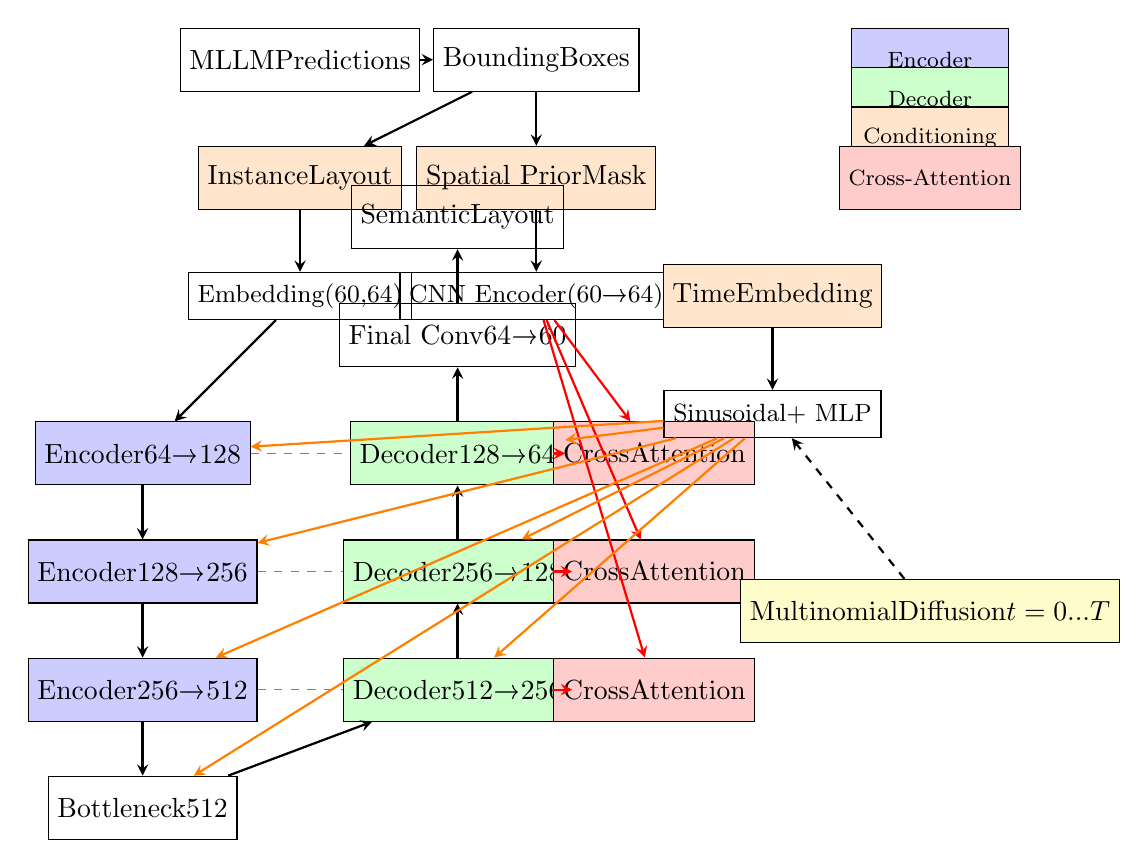
\begin{tikzpicture}[
        node distance=1.5cm,
        box/.style={rectangle, draw, minimum width=2cm, minimum height=0.8cm, text centered},
        smallbox/.style={rectangle, draw, minimum width=1.5cm, minimum height=0.6cm, text centered, font=\small},
        encoder/.style={box, fill=blue!20},
        decoder/.style={box, fill=green!20},
        conditioning/.style={box, fill=orange!20},
        attention/.style={box, fill=red!20},
        arrow/.style={->,>=stealth,thick}
    ]

    % Input Stage
    \node[box] (mllm) at (0,8) {MLLM\\Predictions};
    \node[box] (bbox) at (3,8) {Bounding\\Boxes};
    \node[conditioning] (instance) at (0,6.5) {Instance\\Layout};
    \node[conditioning] (spatial) at (3,6.5) {Spatial Prior\\Mask};
    
    % Embedding Stage
    \node[smallbox] (embed1) at (0,5) {Embedding\\(60,64)};
    \node[smallbox] (embed2) at (3,5) {CNN Encoder\\(60→64)};
    
    % Main U-Net Architecture
    \node[encoder] (enc1) at (-2,3) {Encoder\\64→128};
    \node[encoder] (enc2) at (-2,1.5) {Encoder\\128→256};
    \node[encoder] (enc3) at (-2,0) {Encoder\\256→512};
    
    \node[box] (bottleneck) at (-2,-1.5) {Bottleneck\\512};
    
    \node[decoder] (dec1) at (2,0) {Decoder\\512→256};
    \node[decoder] (dec2) at (2,1.5) {Decoder\\256→128};
    \node[decoder] (dec3) at (2,3) {Decoder\\128→64};
    
    % Cross-Attention Blocks
    \node[attention] (ca1) at (4.5,0) {Cross\\Attention};
    \node[attention] (ca2) at (4.5,1.5) {Cross\\Attention};
    \node[attention] (ca3) at (4.5,3) {Cross\\Attention};
    
    % Time Embedding
    \node[conditioning] (time) at (6,5) {Time\\Embedding};
    \node[smallbox] (sinusoid) at (6,3.5) {Sinusoidal\\+ MLP};
    
    % Output
    \node[box] (output) at (2,4.5) {Final Conv\\64→60};
    \node[box] (result) at (2,6) {Semantic\\Layout};
    
    % Skip Connections (dashed lines)
    \draw[dashed, gray] (enc3) -- (dec1);
    \draw[dashed, gray] (enc2) -- (dec2);
    \draw[dashed, gray] (enc1) -- (dec3);
    
    % Main Flow Arrows
    \draw[arrow] (mllm) -- (bbox);
    \draw[arrow] (bbox) -- (instance);
    \draw[arrow] (bbox) -- (spatial);
    \draw[arrow] (instance) -- (embed1);
    \draw[arrow] (spatial) -- (embed2);
    
    \draw[arrow] (embed1) -- (enc1);
    \draw[arrow] (enc1) -- (enc2);
    \draw[arrow] (enc2) -- (enc3);
    \draw[arrow] (enc3) -- (bottleneck);
    \draw[arrow] (bottleneck) -- (dec1);
    \draw[arrow] (dec1) -- (dec2);
    \draw[arrow] (dec2) -- (dec3);
    \draw[arrow] (dec3) -- (output);
    \draw[arrow] (output) -- (result);
    
    % Cross-Attention Connections
    \draw[arrow, red] (embed2) -- (ca1);
    \draw[arrow, red] (embed2) -- (ca2);
    \draw[arrow, red] (embed2) -- (ca3);
    \draw[arrow, red] (ca1) -- (dec1);
    \draw[arrow, red] (ca2) -- (dec2);
    \draw[arrow, red] (ca3) -- (dec3);
    
    % Time Embedding Connections
    \draw[arrow] (time) -- (sinusoid);
    \draw[arrow, orange] (sinusoid) -- (enc1);
    \draw[arrow, orange] (sinusoid) -- (enc2);
    \draw[arrow, orange] (sinusoid) -- (enc3);
    \draw[arrow, orange] (sinusoid) -- (bottleneck);
    \draw[arrow, orange] (sinusoid) -- (dec1);
    \draw[arrow, orange] (sinusoid) -- (dec2);
    \draw[arrow, orange] (sinusoid) -- (dec3);
    
    % Noise Process (side annotation)
    \node[box, fill=yellow!20] (noise) at (8,1) {Multinomial\\Diffusion\\$t = 0...T$};
    \draw[arrow, dashed] (noise) -- (sinusoid);
    
    % Legend
    \node[encoder, font=\footnotesize] at (8,8) {Encoder};
    \node[decoder, font=\footnotesize] at (8,7.5) {Decoder};
    \node[conditioning, font=\footnotesize] at (8,7) {Conditioning};
    \node[attention, font=\footnotesize] at (8,6.5) {Cross-Attention};
    
    \end{tikzpicture}
    \caption{Complete architecture for multinomial diffusion-based static scene generation. The pipeline consists of: (1) MLLM predictions converted to spatial conditioning masks, (2) Multi-layer cross-attention conditioning (red arrows) integrated at every decoder layer, (3) U-Net backbone with skip connections (dashed gray), and (4) Time embedding injection (orange arrows) throughout the network.}
    \label{fig:diffusion_architecture}
\end{figure}

\paragraph{1. Conditional Input Preparation}
Given the MLLM-predicted bounding box layout, we construct two key conditioning inputs: a \textit{coarse instance layout} providing spatial structure guidance, and a \textit{spatial prior mask} encoding object class locations as multi-channel binary masks $(B, 60, H, W)$. The instance layout is embedded via \texttt{nn.Embedding(60, 64)}, while the spatial prior is processed through a CNN encoder: \texttt{Conv2d(60→64) → GroupNorm → Mish → Conv2d(64→64)}.

\paragraph{2. Multi-Layer Cross-Attention Conditioning}
Our core architectural innovation replaces traditional single-point conditioning with cross-attention blocks integrated at every decoder layer. Each cross-attention block computes:
\begin{align}
Q &= \text{Linear}(\text{features}) \\
K, V &= \text{Linear}(\text{conditioning}) \\
\text{Attention} &= \text{Softmax}(QK^T/\sqrt{d}) \\
\text{Output} &= \text{Features} + \text{Attention}(V)
\end{align}
This mechanism maintains strong conditioning signals throughout the network depth, preventing signal dilution observed in single-injection approaches.

\paragraph{3. Multinomial Diffusion Process}
The forward diffusion process follows:
\begin{equation}
q(x_t | x_0) = \text{Cat}(x_t | \bar{\alpha}_t \cdot x_0 + (1 - \bar{\alpha}_t)/K \cdot \mathbf{1}_K)
\end{equation}
where $\bar{\alpha}_t$ follows a cosine schedule and $K=60$ semantic classes. The reverse process predicts clean data directly ($x_0$-parameterization):
\begin{align}
p_\theta(x_{t-1} | x_t, c) &= \text{Cat}(x_{t-1} | \theta_{\text{post}}(x_t, \hat{x}_0, c)) \\
\hat{x}_0 &= \text{Softmax}(\text{UNet}_\theta(x_t, t, c))
\end{align}
The training objective minimizes the variational bound:
\begin{equation}
\mathcal{L} = \mathbb{E}_{x,t,c}[\text{KL}(q(x_{t-1}|x_t,x_0) \| p_\theta(x_{t-1}|x_t,c))]
\end{equation}

\paragraph{4. Architecture Specifications}
The U-Net backbone employs 4 encoder levels with channel dimensions $[64, 128, 256, 512]$ and symmetric decoder with skip connections. Cross-attention conditioning is integrated at each of the 7 decoder layers with 8 attention heads per block. Dropout (0.1) is applied after the first ResNet block at each level. The final $1 \times 1$ convolution outputs logits for all 60 semantic classes.

\paragraph{5. Training Data Requirements}
Based on recent advances in few-shot diffusion models, we establish minimum training requirements: \textbf{Practical minimum}: 500-1000 samples total with class-balanced distribution (15-20 samples for major classes, 5-10 for rare classes), achieving 65-75\% pixel accuracy. \textbf{Optimal performance}: 2000-5000 samples achieving 80-90\% accuracy. Training employs curriculum learning, semantic embedding initialization, and class-balanced sampling to maximize performance in low-data regimes.


\subsection{Tasks}

The tasks predicted by the MLLM are a sequence of actions to be performed by the player. %TODO: Add more on GUsT integration.

\section{Implementation}

The implementation of the system is divided into two components — the \textbf{Backend (Python)} and the \textbf{Frontend (Unity)} — which together enable interaction between the MLLM (Gemini 2.5 pro for our case), the multinomial diffusion model and the Unity-based scenario generation environment.

\subsection{Backend (Python) Implementation}

The backend is implemented as an HTTP server in Python that interfaces with the \textit{Gemini 2.5 Pro} MLLM to process requests and manage data flow between the model and the Unity client. 
It exposes four primary \texttt{POST} endpoints:

\begin{itemize}
    \item \textbf{/get\_json} – Generates the initial layout or configuration in JSON format based on user input or scene specifications.
    \item \textbf{/refine\_layout} – Refines the generated layout using the multinomial diffusion model.
    \item \textbf{/get\_3d} – Produces 3D representations or assets produuced by Urban Architect~\cite{lu2024urban}.
    \item \textbf{/get\_tasks} – Provides task-level metadata or scenario instructions to GUsT-3D
\end{itemize}

\subsection{Frontend (Unity) Implementation}

The frontend is developed as a part of existing GUsT-3D add-on. It communicates with the Python backend via HTTP, sending requests to the defined endpoints and parsing the responses to generate the scenarios within Unity. 

\section*{Appendix}

\section{Examples}

\subsection{Layout JSON}
\label{app:examples:example_json}

\begin{verbatim}
{
  "static_layout": [
    {
      "id": 1,
      "type": "road",
      "position": [
        250,
        250
      ],
      "size": [
        500,
        20
      ],
      "orientation": 0,
      "layer": "Ground"
    },
    {
      "id": 2,
      "type": "road",
      "position": [
        250,
        250
      ],
      "size": [
        20,
        500
      ],
      "orientation": 90,
      "layer": "Ground"
    },
    {
      "id": 3,
      "type": "sidewalk",
      "position": [
        250,
        230
      ],
      "size": [
        500,
        10
      ],
      "orientation": 0,
      "layer": "Ground"
    },
    {
      "id": 4,
      "type": "sidewalk",
      "position": [
        250,
        270
      ],
      "size": [
        500,
        10
      ],
      "orientation": 0,
      "layer": "Ground"
    },
    {
      "id": 5,
      "type": "sidewalk",
      "position": [
        230,
        250
      ],
      "size": [
        10,
        500
      ],
      "orientation": 90,
      "layer": "Ground"
    },
    {
      "id": 6,
      "type": "sidewalk",
      "position": [
        270,
        250
      ],
      "size": [
        10,
        500
      ],
      "orientation": 90,
      "layer": "Ground"
    },
    {
      "id": 7,
      "type": "building",
      "position": [
        50,
        50
      ],
      "size": [
        100,
        100
      ],
      "orientation": 0,
      "layer": "Wall"
    },
    {
      "id": 8,
      "type": "building",
      "position": [
        450,
        50
      ],
      "size": [
        100,
        100
      ],
      "orientation": 0,
      "layer": "Wall"
    },
    {
      "id": 9,
      "type": "building",
      "position": [
        50,
        450
      ],
      "size": [
        100,
        100
      ],
      "orientation": 0,
      "layer": "Wall"
    },
    {
      "id": 10,
      "type": "building",
      "position": [
        450,
        450
      ],
      "size": [
        100,
        100
      ],
      "orientation": 0,
      "layer": "Wall"
    },
    {
      "id": 11,
      "type": "traffic light",
      "position": [
        240,
        220
      ],
      "size": [
        2,
        5
      ],
      "orientation": 0,
      "layer": "Interactable"
    },
    {
      "id": 12,
      "type": "traffic light",
      "position": [
        260,
        280
      ],
      "size": [
        2,
        5
      ],
      "orientation": 180,
      "layer": "Interactable"
    },
    {
      "id": 13,
      "type": "traffic light",
      "position": [
        220,
        260
      ],
      "size": [
        2,
        5
      ],
      "orientation": 270,
      "layer": "Interactable"
    },
    {
      "id": 14,
      "type": "traffic light",
      "position": [
        280,
        240
      ],
      "size": [
        2,
        5
      ],
      "orientation": 90,
      "layer": "Interactable"
    },
    {
      "id": 15,
      "type": "vegetation",
      "position": [
        150,
        150
      ],
      "size": [
        5,
        5
      ],
      "orientation": 0,
      "layer": "Environment"
    },
    {
      "id": 16,
      "type": "vegetation",
      "position": [
        350,
        150
      ],
      "size": [
        5,
        5
      ],
      "orientation": 0,
      "layer": "Environment"
    },
    {
      "id": 17,
      "type": "vegetation",
      "position": [
        150,
        350
      ],
      "size": [
        5,
        5
      ],
      "orientation": 0,
      "layer": "Environment"
    },
    {
      "id": 18,
      "type": "vegetation",
      "position": [
        350,
        350
      ],
      "size": [
        5,
        5
      ],
      "orientation": 0,
      "layer": "Environment"
    },
    {
      "id": 19,
      "type": "ground",
      "position": [
        250,
        250
      ],
      "size": [
        20,
        20
      ],
      "orientation": 0,
      "layer": "Ground"
    }
  ],
  "dynamic_layout": {
    "trajectories": [
      {
        "id": 101,
        "type": "car",
        "initial_position": [
          100,
          250
        ],
        "layer": "Movable",
        "trajectory_description": [
          {
            "time": 0.0,
            "position": [
              100,
              250
            ]
          },
          {
            "time": 0.5,
            "position": [
              250,
              250
            ]
          },
          {
            "time": 0.7,
            "position": [
              250,
              235
            ]
          },
          {
            "time": 0.9,
            "position": [
              265,
              250
            ]
          }
        ]
      },
      {
        "id": 102,
        "type": "car",
        "initial_position": [
          250,
          400
        ],
        "layer": "Movable",
        "trajectory_description": [
          {
            "time": 0.0,
            "position": [
              250,
              400
            ]
          },
          {
            "time": 0.5,
            "position": [
              250,
              250
            ]
          },
          {
            "time": 0.7,
            "position": [
              235,
              250
            ]
          },
          {
            "time": 0.9,
            "position": [
              250,
              265
            ]
          }
        ]
      },
      {
        "id": 103,
        "type": "bicycle",
        "initial_position": [
          300,
          230
        ],
        "layer": "Movable",
        "trajectory_description": [
          {
            "time": 0.0,
            "position": [
              300,
              230
            ]
          },
          {
            "time": 0.3,
            "position": [
              300,
              250
            ]
          },
          {
            "time": 0.6,
            "position": [
              250,
              250
            ]
          },
          {
            "time": 0.8,
            "position": [
              235,
              250
            ]
          }
        ]
      },
      {
        "id": 104,
        "type": "person",
        "initial_position": [
          300,
          215
        ],
        "layer": "Movable",
        "trajectory_description": [
          {
            "time": 0.0,
            "position": [
              300,
              215
            ]
          },
          {
            "time": 0.3,
            "position": [
              300,
              230
            ]
          },
          {
            "time": 0.6,
            "position": [
              300,
              250
            ]
          },
          {
            "time": 0.8,
            "position": [
              300,
              270
            ]
          }
        ]
      }
    ]
  },
  "tasks": [
    {
      "id": 1,
      "goal": {
        "type": "go",
        "target": "sidewalk_300.0_230.0",
        "key_item": null
      },
      "constraints": {
        "precedence": [],
        "evaluation": "arrive_at_target"
      },
      "help": {
        "baseline": "Head towards the sidewalk to wait for the cyclist.",
        "target": "Reach the designated waiting area.",
        "failure": "Do not enter the road until safe."
      },
      "failure_condition": {
        "type": "collision",
        "item": "car"
      },
      "instructions": {
        "text_en": "Go to the sidewalk at [300, 230] and wait.",
        "text_fr": "Allez sur le trottoir \u00e0 [300, 230] et attendez."
      },
      "trigger": {
        "object_id": 3,
        "function": "on_reach"
      }
    },
    {
      "id": 2,
      "goal": {
        "type": "interact",
        "target": "traffic_light_11",
        "key_item": null
      },
      "constraints": {
        "precedence": [
          1
        ],
        "evaluation": "light_green"
      },
      "help": {
        "baseline": "Observe the traffic light and wait for it to turn green.",
        "target": "Wait for the pedestrian signal to be green.",
        "failure": "Crossing on red is dangerous."
      },
      "failure_condition": {
        "type": "violation",
        "item": "traffic_light"
      },
      "instructions": {
        "text_en": "Wait for the traffic light at [240, 220] to turn green before proceeding.",
        "text_fr": "Attendez que le feu de circulation \u00e0 [240, 220] passe au vert."
      },
      "trigger": {
        "object_id": 11,
        "function": "on_light_green"
      }
    },
    {
      "id": 3,
      "goal": {
        "type": "go",
        "target": "road_250.0_250.0",
        "key_item": null
      },
      "constraints": {
        "precedence": [
          2
        ],
        "evaluation": "arrive_at_target"
      },
      "help": {
        "baseline": "Cross the intersection carefully.",
        "target": "Cross the road safely.",
        "failure": "Avoid vehicles."
      },
      "failure_condition": {
        "type": "collision",
        "item": "car"
      },
      "instructions": {
        "text_en": "Cross the intersection at [250, 250] when the light is green.",
        "text_fr": "Traversez l'intersection \u00e0 [250, 250] lorsque le feu est vert."
      },
      "trigger": {
        "object_id": 19,
        "function": "on_reach_road"
      }
    },
    {
      "id": 4,
      "goal": {
        "type": "go",
        "target": "sidewalk_270.0_250.0",
        "key_item": null
      },
      "constraints": {
        "precedence": [
          3
        ],
        "evaluation": "arrive_at_target"
      },
      "help": {
        "baseline": "Continue across the intersection to the other side.",
        "target": "Reach the other sidewalk.",
        "failure": "Stay on the pedestrian path."
      },
      "failure_condition": {
        "type": "collision",
        "item": "car"
      },
      "instructions": {
        "text_en": "Continue to the sidewalk at [270, 250].",
        "text_fr": "Continuez vers le trottoir \u00e0 [270, 250]."
      },
      "trigger": {
        "object_id": 6,
        "function": "on_reach"
      }
    }
  ]
}
\end{verbatim}



\section{Misc}

\subsection{Meeting Notes}

\subsubsection{01/08/2025}    

\begin{itemize}
    \item \textbf{Clarify Image Usage:} Specify what kinds of images are being referred to in the input for the models (e.g., diagrams, real-world photos, layouts).
    
    \item \textbf{Add details on scenegraph:} Provide more information about the scenegraphs (e.g., format, usage, etc.) in the context of the models.
    
    \item \textbf{Avoid Overly High-Level Descriptions:} Some explanations are too abstract.
    
    \item \textbf{Improve Focus on Vocabulary:} Review and refine terminology. Ensure technical or domain-specific terms are clearly defined and used consistently.
    
    \item \textbf{Identify and Specify Missing Interaction Types:} Clearly outline which user/system interactions are missing or underexplored.
    
    \item \textbf{Sharpen Research Question (RQ):} Make the RQ more concrete.
    
    \item \textbf{Better Categorization of Literature:} Reorganize cited papers using clear categories such as research themes, methodologies, etc.
\end{itemize}

\subsubsection{14/08/2025}    

\begin{itemize}
    \item \textbf{RQ still too high level:} Provide more information about the scenegraphs (e.g., format, usage, etc.) in the context of the models.
    
    \item \textbf{Clarify the missing pieces in the SOTA:} 

    \item \textbf{How to address:} diversity -> generative models, realism -> ontology, dynamic -> tasks
    
    \item \textbf{Start with WorkPlan:}     
    
    \item \textbf{Remove relation between GUsT-3D and generation}
    
\subsubsection{04/09/2025}    

\begin{itemize}
    \item \textbf{Semantic Information Missing:} Find a way to match the scene to Kitti's prior.
    
    \item \textbf{Input unclear:} Scenegraph requires too much information. Need to simplify the input.

    \item \textbf{Use Layout:} Graphdreamer based score distillation doesn't work, use layout instead.
\end{itemize}
\end{itemize}

\subsubsection{29/09/2025}    

\begin{itemize}
    \item \textbf{Organize docs and notes:} Clarify the layout preferably with images.
    
    \item \textbf{Add missing citations:} Add missing citations for stuff like scene background generation in the workplan.

    \item \textbf{Detail:} Detail the missing sections more.

    \item \textbf{Git:} Add the code to gitlab.
\end{itemize}

\subsubsection{08/10/2025}    

\begin{itemize}

    \item \textbf{Validate with more prompts:} Validate the system with additional prompts - realistic, illogical, variations of the same prompts, prompts that recreate Florent's scenarios, decomposing prompts which are "difficult" for a pedestrian (jaywalking, parking lot entrance), etc.

    \item \textbf{Add in the doc:} the prompts discussed in the meeting, diffusion architecture, more details on validation, add examples for failure conditions, SOTA on prompt engineering for multimodal content.
    
\end{itemize}

\subsection{Urban Scenario Generation}

This section discusses pre-existing models used for generating scenarios in urban environments. These models can be broadly classified into procedural and deep generative approaches.

\subsubsection{Procedural Methods}

Procedural methods leverage algorithms and rules to generate urban scenarios, often resulting in highly customizable environments. They can be further divided into two categories:

\paragraph{Classic Procedural Generation} use rules or constraints to generate scenes. The most popular procedural approach used for urban scenarios is Scenic~\cite{fremont2019scenic}, which allows users to define scenarios using a probabilistic programming language. Similarly, MetaUrban~\cite{wu2024metaurban} is a popular urban scenario generation framework to create urban micromobility scenarios using the Metadrive~\cite{li2022metadrive} simulator.

\paragraph{LLM-based Procedural Generation} can be used to enhance procedural generation with natural language understanding. For example, ScenicNL~\cite{elmaaroufi2024scenicnl} and ChatScene~\cite{zhang2024chatscene} use LLMs to generate scenic code from prompts and then define the scenarios in Scenic. TTSG\cite{ruan2024traffic} is another framework that uses an to plan a traffic scenario using an LLM in JSON and then render it using CARLA~\cite{dosovitskiy2017carla}. CityX~\cite{zhang2024cityx} is multi-agent framework that uses LLM to assemble assets using the procedural content generation (PCG) library as well as plan actions for the agents in the scenario.

Even though procedural approaches can be highly customizable and allow for precise control over the generated scenarios, they typically suffer from a lack of realism, as they rely on predefined rules that may not capture the full complexity of real-world environments. However, they can be useful in creating diverse scenarios that adhere to specific constraints or requirements. For example, a scenario with a crossroad with a specific number of lanes, a certain type of road surface, and a defined layout of buildings. However, no real crossroad would exist in the world that conforms to these specifications.

\subsubsection{Deep-Generative Methods}

Deep-Generative Approaches have recently become popular for various sorts of 3D generation. To create a complete scenario, some techniques use generative models such as GANs, VAEs or Diffusion models in combination with procedural techniques. These can be broadly classified into the following categories:

\paragraph{Procedural Environments with Deep-Generative Dynamics} generate the static aspects of the environment using procedural techniques, while the dynamic aspects such as vehicles and pedestrians are generated using generative models. For example, Chatdyn~\cite{wei2024chatdyn} uses CARLA~\cite{dosovitskiy2017carla} to construct the traffic environment, then populate it with pedestrians and vehicles, each equipped with an LLM agent to generate a high-level scenario plan. This high-level plan is then executed in a low-level PedExecutor using Text2Motion~\cite{guo2024momask} for pedestrians and VehExectutor using a physics-based, history-aware reinforcement learning controller to produce vehicle trajectories.

\paragraph{Procedural Dynamics with Deep-Generative Environments} generate the dynamic aspects such as vehicles and pedestrians using procedural techniques. UrbanWorld~\cite{shang2024urbanworld} converts 2.5D urban layout data into a structured 3D city with separated assets, applying depth-aware, multi-view diffusion-based texture rendering and UV inpainting to achieve high-fidelity visuals. It also uses an urban MLLM for designing the world and provides dynamic elements which are planned using a random tree path planning algorithm. CityDreamer4D~\cite{xie2024citydreamer} modularly integrates autoregressive token-based generation, neural rendering (e.g., NeRF-style volumetrics), and procedural traffic modeling to synthesize large-scale, time-varying 3D cities.

\paragraph{Complete Deep-Generative Approaches} recreate the static as well as the dynamic aspects using the learnt representation. Infinicube~\cite{lu2024infinicube} constructs a large, dynamic 3D voxel world from input HD maps, vehicle positions, and text prompts; then, it generates photorealistic driving videos and reconstructs the scene into a manipulable 3D environment by fusing voxel- and video-based representations. UniScene~\cite{li2025uniscene} UniScene generates driving scenes in three modalities—semantic occupancy, multi-view video, and LiDAR—by first producing a controllable, temporally consistent occupancy sequence from BEV layouts. This occupancy then serves as unified geometric–semantic guidance to synthesize realistic videos and point clouds, ensuring cross-modal consistency and editability.

\subsection{Scenegraph-Controlled Diffusion}

Despite the advancements in urban scenario generation, very few methods have explored the use of scenegraphs to control the generation process. In recent years, the achievements in text-to-image generation has enabled the advancement of text-to-3D generation using Score Distillation Sampling (SDS)~\cite{poole2022dreamfusion} which optimizes a 3D model by aligning 2D images rendered at arbitrary viewpoints with the distribution derived from a text-conditioned diffusion model. Subsequent works including ProlificDreamer~\cite{wang2023prolificdreamer} introduced Variational Score Distillation (VSD) which addresses the over-regularization and mode collapse issues of SDS by introducing a variational formulation that jointly optimizes the 3D representation and a learnable Gaussian noise distribution, enabling more faithful geometry and richer texture generation. GraphDreamer~\cite{gao2024graphdreamer}  uses the the SDS process with scenegraphs to enable more structured and controllable scene generation. However, it uses a simplified static scenegraph representation as shown in Visual genome~\cite{krishna2017visual} in which, nodes represent the objects in the scene, edges represent the relationship between these nodes and attriubtes represent the properties of the node. Example, Elderly (attribute) man (Node) wearing (edge) a hat(node). This limits the ability to generate dynamic scenarios where the relationships between objects change over time.


\subsection{Scenegraph-guided Generation}

Scenegraph-guided 3D generation is the process of creating 3D environments by leveraging scene graphs, which are structured representations of the objects and their relationships within a scene. A major advantage of scenegraph-guided generation is that it provides a clear relationship between the elements which allows for better generation than other techniques such as simple text prompts or bounding boxes. Scenethesis~\cite{ling2025scenethesis} uses a Vision-Language Model (VLM) to create a scenegraph with parent-child relationships and localizes objects using 3D bounding boxes. Work by Liu et al.~\cite{liu2025controllable} defines scenegraphs as graphs where instance nodes represent countable objects with semantic and positional features, a singleton road node encodes global scene structure, and edges capture both physical proximity among instances and connectivity to the road. X-Scene~\cite{yang2025x} is another work that uses LLMs (Large-Language Models) to create a scenegraph with nodes (objects) and edges (relationships) to facilitate the generation process. Graphdreamer~\cite{gao2024graphdreamer} employs scenegraphs structured around the Visual Genome~\cite{krishna2017visual} format, where nodes represent objects with associated attributes, and edges encode the relationships between these objects to guide the generation process. Despite the advancements in scenegraph-guided generation, all of these works focus on static scenes and do not consider dynamic scenarios where the state of the objects changes over time.

\subsection{Grounding: Input for Scene Generation}

Generative models have already been applied to urban scenario generation, where models synthesize plausible urban environments, pedestrian layouts, or vehicle positions from various types of input. An input in the context of a generative model is any data—such as a prompt, image, or scenario graph—provided to influence the output. Grounding, on the other hand, is the process of linking elements of that input to specific, coherent representations in the generated scenario, such as ensuring the "footpath" appears visually plausible, is correctly positioned on the "road", and respects spatial relationships or physical constraints. Grounding ensures the generated scenario isn't just randomly composed but meaningfully aligned with the intended semantics of the input. The common ways to do grounding are,

\subsubsection{Rules and Constraints}

\paragraph{Rules} can be used to give a prescriptive logic that defines how to generate or modify a scenario. Rule-based systems are necessarily procedural, meaning they follow a set of predefined steps or algorithms to create scenarios. Table \ref{tab:rule_based_models} lists some of the recent rule-based models for scenario generation. Although these systems allow users to define rules for generating scenarios—such as the placement of buildings, roads, and other elements—they often require an intermediate representation which captures the real-world environments. Creating such representations can be challenging, as it requires a deep understanding of the underlying rules and relationships between different elements. Additionally, rule-based systems can be limited in their ability to generate diverse and realistic scenarios, as they rely on predefined rules that may not capture the full complexity of real-world environments.traffic

\begin{table}[ht]
\centering
    \begin{tabular}{|c|c|c|}
    \hline
    \textbf{Model} & \textbf{Technique} & \textbf{Output} \\ \hline
    CityEngine~\cite{parish2001procedural} & Procedural Modeling with Rules & 3D scene \\ \hline
    Infinigen~\cite{raistrick2023infinite} & Procedural Modeling with Rules & 3D scene \\ \hline
    MetaUrban~\cite{wu2024metaurban} & Description Scripts for Scene Layout & 3D Scenario \\ \hline    
    \end{tabular}
\caption{Rule-based Models for Urban Scenario Generation}
\label{tab:rule_based_models}
\end{table}

\paragraph{Constraints} define conditions that must be satisfied to get a valid scenario. Scenic~\cite{fremont2019scenic} is a probabilistic programming language that allows users to define constraints for generating scenarios. It uses a declarative approach to specify the properties of the scenario, such as the layout, objects, and their relationships. These can then be rendered using a frontend such as CARLA~\cite{dosovitskiy2017carla}. However, it suffers from the same limitations of rule-based systems, as it can only generate scenarios that fit within the defined constraints, potentially missing out on the richness and variability of real-world environments.

\subsection{Diffusion-based 4D Generation}

Diffusion models have emerged as a powerful approach for generating high‐quality 3D content by iteratively refining a random noise input into a coherent output. DreamFusion~\cite{poole2022dreamfusion} initially introduced text‐to‐3D synthesis by optimizing a neural radiance field so that rendered views, when noised and denoised by a pretrained text‐conditioned diffusion model, produce identical gradients via Score Distillation Sampling (SDS). This framework was extended to dynamic scenes in MaV3D, which employs video‐based SDS to animate a time‐conditioned radiance field into a 4D scene~\cite{singer2023text}. However, MaV3D’s reliance on a single diffusion prior leads to trade‐offs between appearance fidelity, 3D consistency, and motion realism. 4D‐fy~\cite{bahmani20244d} addresses this by hybridizing three SDS signals—3D‐aware image SDS for geometry, standard image SDS for texture, and video SDS for motion—alternating updates to preserve all three qualities. Animate124~\cite{zhao2023animate124} further refines single‐image animation into 4D using a coarse‐to‐fine 4D grid backbone optimized first with 2D and 3D image priors, then with video diffusion, and finally with a personalized ControlNet fine‐tuning stage to prevent semantic drift. More recently, Trans4D~\cite{zeng2024trans4d} leverages a multimodal large language model to perform physics‐aware 4D scene planning—generating object trajectories, rotations, and transition times—and introduces a Transition Network that predicts point‐wise appearance or disappearance probabilities to realize complex geometry‐aware transitions such as a missile transforming into an explosion cloud. Despite their impressive generative capabilities, these diffusion-based 4D synthesis methods still lack the explicit, structured control afforded by scene graphs, making it difficult to enforce complex object relationships or constraints at generation time.


\subsection{Datasets}

In this section, we review the datasets that are used to train generative models for road crossing scenarios. Table~\ref{tab:datasets} lists some of the datasets commonly used for training and evaluating generative models in urban environments.

\begin{table}[ht]
\centering
\caption{Overview of selected datasets for foundation model-based scenario generation and analysis.}
\label{tab:datasets}
\renewcommand{\arraystretch}{1.1}
\begin{tabular}{lccccccc}
\toprule
\textbf{Dataset} & \textbf{Year} & \textbf{View} & \textbf{Source} \\
\midrule
SIND~\cite{xu2022drone}             & 2022 & BEV        & Real         \\
Waymo Open~\cite{sun2020scalability}       & 2020 & FPV        & Real  \\
Argoverse~\cite{chang2019argoverse}\cite{wilson2023argoverse}        & 2023 & BEV/FPV    & Real \\
nuScenes~\cite{caesar2020nuscenes}      & 2022 & FPV        & Real \\
KITTI~\cite{geiger2012we}            & 2012 & FPV        & Real \\
Cityscapes~\cite{cordts2016cityscapes}      & 2016 & FPV        & .. \\
HoliCity~\cite{zhou2020holicity}          & 2020 & FPV        & .. \\
OmniCity~\cite{li2023omnicity}          & 2023 & FPV        & ..  \\
GoogleEarth~\cite{xie2024citydreamer}          & 2024 & BEV        & Real  \\
OSM~\cite{xie2024citydreamer}          & 2024 & BEV        & Real \\
CarlaSC~\cite{wilson2022motionsc}          & 2022 & BEV/FPV    & Synthetic \\
CityTopia~\cite{xie2025citydreamer4d}          & 2025 & BEV/FPV    & .. \\
\bottomrule
\end{tabular}
\end{table}


\subsection{Input Scenegraph}
We represent a temporal (dynamic) scenegraph as a tuple
\begin{equation}
S = (V, E, \mathcal{T}, \tau)
\end{equation}
where
\begin{itemize}
    \item $V = \{v_i\}_{i=1}^N$ is a finite set of nodes (objects). Each node $v_i$ is itself a tuple
    \begin{equation}
        v_i = \big(\mathrm{id}_i, \mathcal{A}_i^{\mathrm{static}}, \{(I_{i,k}, \mathcal{A}_i^{\mathrm{dynamic}}|_{I_{i,k}})\}_{k=1}^{K_i} \big),
    \end{equation}
    where
    \begin{itemize}
        \item $\mathrm{id}_i$ is a unique identifier (string),
        \item $\mathcal{A}_i^{\mathrm{static}}$ is the attribute map for invariant attributes:
        \[
        \mathcal{A}_i^{\mathrm{static}} : K_\mathrm{static} \rightharpoonup V,
        \]
        e.g., type, material,
        \item $\{(I_{i,k}, \mathcal{A}_i^{\mathrm{dynamic}}|_{I_{i,k}})\}$ is an ordered set of temporal states where each
        \[
        I_{i,k} = [t_{i,k}(0), t_{i,k}(1)] \subseteq \mathcal{T}
        \]
        is a closed time interval, and $\mathcal{A}_i^{\mathrm{dynamic}}|_{I_{i,k}}$ are the dynamic attribute values valid for that interval (e.g., position, lid state, traffic-light color).
    \end{itemize}
    \item $E \subseteq V \times V$ is a set of directed edges. Each edge $e = (v_i, v_j)$ is augmented by
    \begin{equation}
        e = (v_i, v_j, r_{ij}, C_{ij}),
    \end{equation}
    where
    \begin{itemize}
        \item $v_i$ is the source node,
        \item $v_j$ is the target node,
        \item $r_{ij}$ is the relation type (e.g., ``next\_to'', ``controls''),
        \item $C_{ij}$ is an optional constraint function mapping dynamic attributes of $v_i$ to changes in $v_j$ (e.g., if traffic light changes to red, car stops).
    \end{itemize}
    \item $\mathcal{T}$ is the global time domain.
    \item $\tau: \bigcup_i \mathcal{S}_i \cup \bigcup_{i,j} \mathcal{I}_{ij} \to \mathcal{P}$ is an optional grounding map to represent the dynamic aspects w.r.t.\ time.
\end{itemize}

\paragraph{Semantics}  
A dynamic scenegraph $S$ encodes both
\begin{enumerate}
    \item the \emph{static layout} through static attributes $\mathcal{A}_i^{\mathrm{static}}$ and relations $r_{ij}$ that are continuously active (or active on $\mathcal{T}$),
    \item the \emph{dynamic behaviour} through temporal attributes $\mathcal{A}_i^{\mathrm{dynamic}}$ and constraint relations $C_{ij}$ between nodes.
\end{enumerate}

\subsubsection*{Example}
Figure \ref{fig:dynamic_scenegraph_example} illustrates the example dynamic scenegraph.

\begin{figure}[ht]
\centering
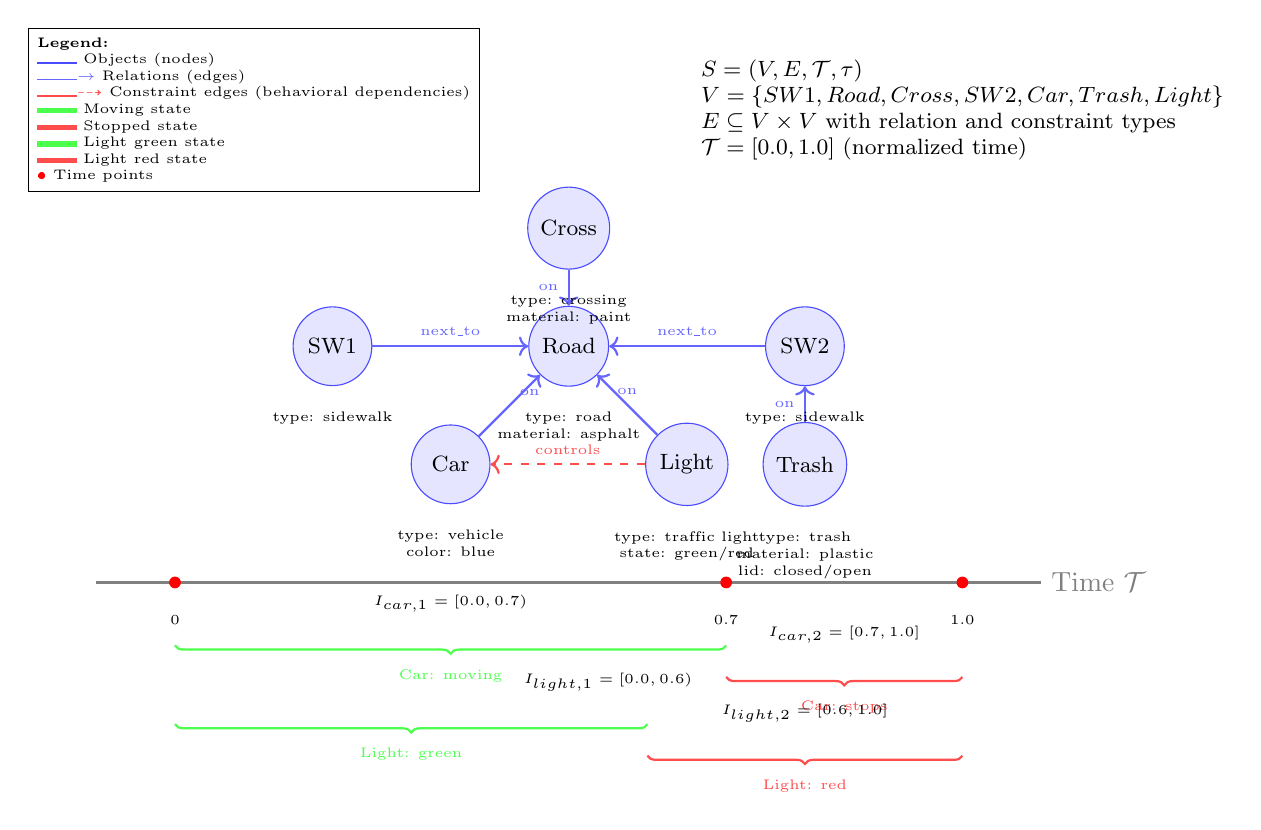
\begin{tikzpicture}[
    object/.style={circle, draw=blue!70, fill=blue!10, minimum size=1cm, font=\footnotesize},
    relation/.style={->, thick, blue!60},
    constraint/.style={->, thick, red!70, dashed},
    timeaxis/.style={thick, gray},
    timepoint/.style={circle, fill=red, inner sep=1.5pt},
    attr/.style={font=\tiny, align=center}
]
% Time axis
\draw[timeaxis] (-1,0) -- (11,0) node[right] {Time $\mathcal{T}$};
\foreach \t in {0,0.7,1.0} {
    \node[timepoint] at ({\t*10},0) {};
    \node[below, font=\tiny] at ({\t*10},-0.3) {\t};
}

% Nodes
\node[object] (sidewalk1) at (2,3) {SW1};
\node[object] (road) at (5,3) {Road};
\node[object] (crossing) at (5,4.5) {Cross};
\node[object] (sidewalk2) at (8,3) {SW2};
\node[object] (car) at (3.5,1.5) {Car};
\node[object] (trash) at (8,1.5) {Trash};
\node[object] (light) at (6.5,1.5) {Light};

% Temporal states visualization
\draw[thick, green!70, decoration={brace,amplitude=3pt,mirror}, decorate]
(0,-0.8) -- (7,-0.8) node[midway,below=5pt,font=\tiny] {Car: moving};
\draw[thick, red!70, decoration={brace,amplitude=3pt,mirror}, decorate]
(7,-1.2) -- (10,-1.2) node[midway,below=5pt,font=\tiny] {Car: stops};
\draw[thick, green!70, decoration={brace,amplitude=3pt,mirror}, decorate]
(0,-1.8) -- (6,-1.8) node[midway,below=5pt,font=\tiny] {Light: green};
\draw[thick, red!70, decoration={brace,amplitude=3pt,mirror}, decorate]
(6,-2.2) -- (10,-2.2) node[midway,below=5pt,font=\tiny] {Light: red};

% Relations
\draw[relation] (sidewalk1) -- (road) node[midway,above,attr] {next\_to};
\draw[relation] (sidewalk2) -- (road) node[midway,above,attr] {next\_to};
\draw[relation] (crossing) -- (road) node[midway,left,attr] {on};
\draw[relation] (car) -- (road) node[midway,above right,attr] {on};
\draw[relation] (trash) -- (sidewalk2) node[midway,left,attr] {on};
\draw[relation] (light) -- (road) node[midway,above,attr] {on};

% Constraint
\draw[constraint] (light) -- (car) node[midway,above,red!70,attr] {controls};

% Attributes
\node[attr, below=0.2cm of sidewalk1] {type: sidewalk};
\node[attr, below=0.2cm of road] {type: road\\material: asphalt};
\node[attr, below=0.2cm of crossing] {type: crossing\\material: paint};
\node[attr, below=0.2cm of sidewalk2] {type: sidewalk};
\node[attr, below=0.2cm of car] {type: vehicle\\color: blue};
\node[attr, below=0.2cm of trash] {type: trash\\material: plastic\\lid: closed/open};
\node[attr, below=0.2cm of light] {type: traffic light\\state: green/red};

% Temporal intervals
\node[font=\tiny, above] at (3.5,-0.5) {$I_{car,1} = [0.0, 0.7)$};
\node[font=\tiny, above] at (8.5,-0.9) {$I_{car,2} = [0.7, 1.0]$};
\node[font=\tiny, above] at (5.5,-1.5) {$I_{light,1} = [0.0, 0.6)$};
\node[font=\tiny, above] at (8,-1.9) {$I_{light,2} = [0.6, 1.0]$};

% Scene graph equation annotation
\node[align=left, font=\footnotesize] at (10,6) {
$S = (V, E, \mathcal{T}, \tau)$\\
$V = \{SW1, Road, Cross, SW2, Car, Trash, Light\}$\\
$E \subseteq V \times V$ with relation and constraint types\\
$\mathcal{T} = [0.0, 1.0]$ (normalized time)
};

% Legend
\node[align=left, font=\tiny, draw, fill=white] at (1,6) {
\textbf{Legend:}\\
\textcolor{blue!70}{\rule{0.5cm}{0.5pt}} Objects (nodes)\\
\textcolor{blue!60}{\rule{0.5cm}{0.5pt}$\rightarrow$} Relations (edges)\\
\textcolor{red!70}{\rule{0.5cm}{0.5pt}$\dashrightarrow$} Constraint edges (behavioral dependencies)\\
\textcolor{green!70}{\rule{0.5cm}{2pt}} Moving state\\
\textcolor{red!70}{\rule{0.5cm}{2pt}} Stopped state\\
\textcolor{green!70}{\rule{0.5cm}{2pt}} Light green state\\
\textcolor{red!70}{\rule{0.5cm}{2pt}} Light red state\\
\textcolor{red}{\textbullet} Time points
};
\end{tikzpicture}
\caption{Example dynamic scenegraph with constraints (nodes, relations with active intervals, temporal states, and dependency edges).}
\label{fig:dynamic_scenegraph_example}
\end{figure}


\bibliographystyle{abbrv}
\bibliography{main}

\end{document}